三角函数求导所用的基本极限，可以直接由单位圆的面积比较建立。图\ref{fv:c1:sine}取 $0<h<\pi/2$，$OA=OB=1$，$AT$为圆的切线。三角形 $OAB$包含在扇形 $OAB$内，扇形又包含在三角形 $OAT$内，因此
\[
 \tfrac12\sin h<\tfrac12h<\tfrac12\tan h,
 \qquad \cos h<\frac{\sin h}{h}<1.
\]
\fig{fv:c1:sine}{以弧度表示扇形面积，才能把几何夹逼写成极限}{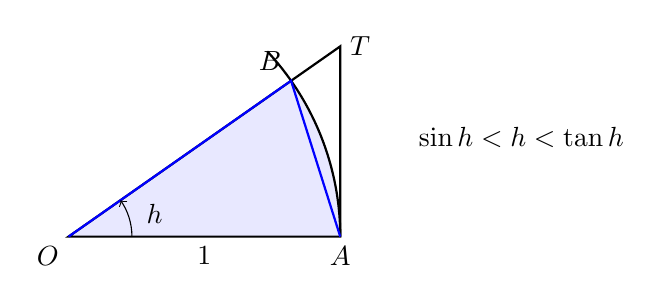
\begin{tikzpicture}[scale=1.15]
\coordinate(O)at(0,0);\coordinate(A)at(3,0);\coordinate(B)at(2.457,1.721);\coordinate(T)at(3,2.101);
\fill[blue!9](O)--(A)arc(0:35:3)--cycle;
\draw[thick](O)--(A)--(T)--cycle;\draw[thick](A)arc(0:43:3);\draw[blue,thick](O)--(B)--(A);
\draw[->](.7,0)arc(0:35:.7);\node at(.95,.25){$h$};
\node[below left]at(O){$O$};\node[below]at(A){$A$};\node[above left]at(B){$B$};\node[right]at(T){$T$};
\node[below]at(1.5,0){$1$};\node at(5,1.1){$\sin h<h<\tan h$};
\end{tikzpicture}}
当 $h\to0^+$，两端均趋于一；$\sin h/h$是偶函数，左极限相同，故极限为一。图中的 $h$必须是弧度数，否则扇形面积不等于 $h/2$。同时 $(1-\cos h)/h=\sin^2h/[h(1+\cos h)]\to0$，于是求导推导所需的两个极限都有了依据。
